\documentclass[final,3p,times,twocolumn]{elsarticle}
\usepackage{amsmath,amssymb,graphicx,booktabs,multirow,url}
\usepackage{fontspec}
\setmainfont{Times New Roman}
\setsansfont{Helvetica}
\setmonofont{Courier New}
\graphicspath{{figures/}}
\newenvironment{widefigure}[1][t]{\begin{figure*}[#1]}{\end{figure*}}
\newenvironment{widetable}[1][t]{\begin{table*}[#1]}{\end{table*}}
\newcommand{\myna}{\textsc{Myna}}
\newcommand{\stream}{\textsc{Myna-Stream}}
\newcommand{\vsix}{\textsc{Myna-v6}}
\journal{Elsevier}
\begin{document}
\begin{frontmatter}
\title{Myna: A Measurement Study of Typed Agent Decision Engines}
\author[1]{Aashish Kumar Mahato\corref{cor1}}
\author[2]{Prakrist Dhakal}
\affiliation[1]{organization={Independent Researcher}, city={Kathmandu}, country={Nepal}}
\affiliation[2]{organization={Independent Researcher}, state={North Carolina}, country={USA}}
\tnotetext[1]{Graduate of Vellore Institute of Technology (VIT), Vellore, India. This work was conducted independently after graduation. A. K. Mahato: ORCID 0009-0007-8952-6357. P. Dhakal: ORCID 0009-0000-9463-0094.}
\cortext[cor1]{First and corresponding author.}
\begin{abstract}
Typed decision engines score a fixed option set instead of generating text. This paper reports a measurement study of Myna, two engines behind one typed choice/score/noul contract: a 14.45M gated-linear-attention streaming engine with a 576 KiB state, and a 446.63M fine-tuned DeBERTa-v3-large with a cardinality-routed readout. On a frozen 16-cell suite (1,176 bundles, 1,440 questions) Myna v6 reaches 0.8620 macro against five external systems: a supervised TF-IDF classifier (0.7111), three configurations of Laya 0.4.19 (0.7050 best), VegaML 0.15.0 (0.6160), a train-prior majority classifier (0.3726), and a zero-shot NLI scorer (0.3278). The comparison is in-domain for Myna and out-of-domain or zero-shot for the engines, so it is reported as a footing-qualified comparison rather than a leaderboard claim. Three results are bounded or negative. Cardinality routing is a budget repair worth 0.0399 macro on exactly one cell, and the isolated ablation on one checkpoint shows the other 15 cells identical. Cross-question consistency is an observed property of the encoder (3/172 contradictions against 10/172 and 29/172 for the external engines), not an enforced constraint. Split-conformal sets cover 83.68\% at a 90\% target and 93.33\% at 95\%, so the paper reports calibration error (ECE 0.0190) and risk--coverage instead of a guarantee. The streaming arm answers in 33--870 ms with a 576 KiB state and runs in a browser at $1.03\times10^{-6}$ drift. Every figure is recomputed from released per-question records.
\end{abstract}
\begin{keyword}
Decision engines \sep typed decisions \sep cardinality \sep calibration \sep selective prediction \sep conformal prediction \sep gated linear attention \sep edge deployment \sep reproducibility
\end{keyword}
\end{frontmatter}
\section{Introduction}
\label{sec:intro}

An agent that processes tickets, threads, or page states asks many small questions: whether a
message is a refund request, how severe it is, which department owns it. Each question has a
small, fixed answer set, and the state on which it is asked grows with every turn.
Autoregressive language models answer such questions fluently but pay for generation on every
call and can return text outside the option set. A non-autoregressive \emph{decision engine}
instead returns a categorical distribution over predefined options
\cite{li2026jev,duan2026gdm}. The design is attractive for high-frequency routing, but three
properties determine whether it can be deployed: whether the option set fits the model's input
budget, whether the confidence it reports can support abstention, and whether the answers to the
questions of one bundle are mutually consistent.

This paper reports a measurement study of \myna, two engines behind one typed
\texttt{choice}/\texttt{score}/\texttt{noul} contract. The third primitive, \texttt{noul}, is a two-option boolean question over $\{\text{no},\text{yes}\}$; the name is the API's. \stream{} is a 14.45M-parameter
gated-linear-attention engine whose retained state is 576 KiB at every length from 128 to
16{,}384 tokens. \vsix{} is a 446.63M-parameter fine-tuned DeBERTa-v3-large with a
cardinality-routed readout; it re-encodes the state on every question and is the accuracy arm.
The two share the question schema, the answer record, the abstention seam, and the serving API,
and nothing else. A latency measurement on one engine is therefore not a statement about the
other, and the paper keeps the two apart throughout.

The study is conducted on \textsc{decision-v2-pilot}, a frozen suite of 1{,}176 test bundles and
1{,}440 questions over 16 cells drawn from 11 public sources (Table~\ref{tab:dataset}). Every arm
is scored on the same rows, and every aggregate is recomputed from released per-question records
by a single aggregation script shipped with the paper, so a table cannot drift from the records
it cites.

\textbf{Contributions.} The paper makes five contributions, two of them negative results.

\begin{itemize}
\item \textbf{A like-for-row comparison with five external systems.} The same 1{,}176 test
bundles are scored by \vsix{}, by three configurations of a contemporary decision engine
(Laya 0.4.19), by a second engine (VegaML 0.15.0), and by three classical references: a
train-prior majority classifier, a supervised TF-IDF classifier, and a zero-shot NLI scorer.
\vsix{} reaches 0.8620 macro against 0.7111 for TF-IDF, 0.7050 for the best Laya configuration,
0.6160 for VegaML, 0.3726 for the majority classifier, and 0.3278 for NLI. The comparison is
in-domain for \vsix{} and out-of-domain or zero-shot for the others, and
Section~\ref{sec:baselines} states that footing with each number.
\item \textbf{A cardinality-budget diagnosis and an isolated routing ablation.} The packed
layout fits every cell with $K\le15$ options. The 77-way cell overflows on 50 of 116 rows,
consumes 490 option-span tokens (6.36 per option), and collapses. Forcing the packed scorer on
every cell, with the weights held fixed, scores 0.0345 on that cell and 0.8222 macro; enabling
the router on the same weights scores 0.6724 and 0.8620. No other cell changes. Routing is a
budget repair for one cell, worth $+0.0399$ macro, and the paper presents it as such.
\item \textbf{Bundle consistency as a measured property, with both predicates released.} The
checkpoint records 0/172 contradictions. That record is reproduced by the released notebook's rule,
recovered from the released notebook (0/172 for \vsix{}, 1/172 for Laya, 2/172 for VegaML), but
the rule only inspects choice--boolean pairs and cannot see the yelp rating/recommendation case. A
broader released predicate gives 3/172, 10/172, and 29/172. The
cross-question graph head is never called at inference and the ablation is identical with it on,
off or shuffled, so consistency is a property of the fine-tuned encoder rather than an enforced
constraint, and no architectural claim is attached to it.
\item \textbf{A calibration and conformal audit.} Temperature scaling gives ECE 0.0190 and a
multiclass Brier score of 0.0449 on the 1{,}440 test questions, with selective accuracy 0.9815 at
60\% coverage. Split-conformal sets cover 83.68\% at a 90\% target and 93.33\% at 95\%, so the
paper reports the undercoverage and uses calibration and risk--coverage for abstention instead of
a coverage guarantee.
\item \textbf{A systems study of the streaming arm.} On one Apple M5, \stream{} answers in
33--870 ms with a state that does not grow, ports to MLX at 1.76--2.40$\times$ over PyTorch MPS,
and runs in Chrome/WebAssembly at $1.03\times10^{-6}$ maximum probability drift. int8 is 3.17$\times$
smaller but not faster and not faithful, so fp32 is deployed on both routes.
\end{itemize}

Section~\ref{sec:related} positions the work, Section~\ref{sec:contract} defines the contract and
the two engines, and Sections~\ref{sec:cardinality}--\ref{sec:diagnostics} report the
measurements, and Section~\ref{sec:limitations} states what the study does not establish.

\section{Related Work}
\label{sec:related}

\textbf{Typed and zero-shot decision models.}
Cloze-style reformulation turns classification into scoring option strings
\cite{schick2021pet}, and prompt-based fine-tuning with demonstrations improves few-shot
performance \cite{gao2021lmbff}. Entailment-based zero-shot classification scores labels as
hypotheses \cite{yin2019benchmarking}; SetFit shows that sentence-encoder fine-tuning is
competitive with prompts at small label budgets \cite{tunstall2022setfit}. The recent \emph{Jev}
line makes the decision-model framing explicit: a model returns a categorical distribution over
predefined options without generating text \cite{li2026jev}, and JEVal benchmarks that family
across 36 datasets \cite{duan2026gdm}. JEVal's findings motivate the calibration question:
decision models can identify the likely outcome while substantially overstating its probability.
The suite studied here is smaller and the accuracy arm is in-domain, but the failure modes are
the same.

\textbf{External baselines.}
The comparison set spans two contemporary decision engines and three classical references. The
classical references are a train-prior majority classifier, a TF-IDF unigram/bigram classifier
with logistic regression, and a zero-shot NLI scorer applied in the entailment tradition of
\cite{yin2019benchmarking}. The two engines are evaluated by their own released harnesses on the
same rows. None of the five is a like-for-like training-budget comparison with a fine-tuned
encoder, and Section~\ref{sec:baselines} treats the footing as part of each number.

\textbf{Efficient sequence models.}
Linear attention replaces the quadratic attention matrix with a recurrence whose state is fixed
in size \cite{katharopoulos2020transformers}; gated linear attention adds a data-dependent forget
gate and hardware-efficient training \cite{yang2024gla}. State-space models such as Mamba
\cite{gu2024mamba} and RWKV \cite{peng2023rwkv} make the same trade, and IO-aware exact attention
\cite{dao2022flashattention} and sparse attention \cite{beltagy2020longformer} attack the cost
from other directions. The streaming arm is a six-layer gated-linear-attention trunk; the
citations are lineage and motive, not a claim of a new architecture.

\textbf{Calibration, selective prediction, and conformal sets.}
Temperature scaling and reliability diagrams are the standard calibration tools
\cite{guo2017calibration}; modern networks remain miscalibrated under dataset shift
\cite{ovadia2019uncertainty}. Selective classification trades coverage for risk
\cite{geifman2017selective,geifman2019selectivenet}. Split conformal prediction gives
distribution-free marginal coverage under exchangeability
\cite{lei2018distribution,angelopoulos2021gentle}, and conformalized quantile regression reports
coverage and interval length together \cite{romano2019cqr}. Empirical coverage below nominal is a
known consequence of violated exchangeability, and the diagnostic is to report coverage by
subgroup rather than to withdraw the method silently; Section~\ref{sec:calibration} follows that
practice and concludes that the sets are not usable for abstention on this suite.

\textbf{Cascades, edge deployment, and quantization.}
Early-exit networks decide per input how much computation to spend
\cite{teerapittayanon2016branchynet,xin2020fastbert,zhou2020deebert}. Post-training quantization
reduces bytes but can move probabilities
\cite{dettmers2022llmint8,frantar2023gptq,xiao2023smoothquant}. The two-engine design is a coarse
cascade: the constant-state engine handles frequent decisions and the cross-encoder is the
accuracy arm. The paper measures the two ends and the portability of the small end, not a joint
deferral policy.

\textbf{Measurement and reproducibility.}
Scoring errors in evaluation harnesses are a recurring source of overstated results, and the
usual remedy is to recompute every aggregate from released per-item records rather than from a
summary table. This paper adopts that discipline: its aggregation script refuses a record whose
correctness flag disagrees with its own prediction and gold, so a table cannot drift from the
records it cites.

The packed-versus-decoupled choice is the classical reranking trade-off. Poly-encoders
\cite{humeau2020poly} and late-interaction models such as ColBERT \cite{khattab2020colbert} encode
the context once and score many candidates cheaply, which is the $O(1)$-pass side; cross-encoders
score each pair jointly, which is the $O(K)$ side our set-aware head occupies. Extreme
multi-class classification addresses the same $K\gg16$ regime with label embeddings rather than
$K$ forward passes. Our routing is the crude end of that spectrum, chosen because the deployed
encoder is fixed; the measurements in Section~\ref{sec:cardinality} bound what it buys.

\section{The Decision Contract and Two Engines}
\label{sec:contract}

\subsection{The typed contract}
A \emph{bundle} is a state $x$ and a set of questions $Q=\{q_1,\dots,q_m\}$. Each question has a
type $\tau\in\{\texttt{choice},\texttt{score},\texttt{noul}\}$ and an option set $O_q$ with
cardinality $K_q=|O_q|$. A \texttt{choice} returns one option; a \texttt{score} returns a level
and an expected score; a \texttt{noul} returns $p(\text{yes})$. Every answer carries a probability
vector, a confidence, a 90\% conformal set, an abstention flag, and the routing mode that produced
it. The contract is the same for both engines; only the scorer behind it changes.

\subsection{Formal description}
\label{sec:formal}

\emph{Notation.} A bundle is a token sequence $x=(x_1,\dots,x_T)$ and questions
$Q=\{q_1,\dots,q_m\}$. Question $q$ has type $\tau\in\{\textsc{choice},\textsc{score},
\textsc{noul}\}$ and an ordered option set $O_q=(o_1,\dots,o_K)$. \textsc{choice} selects an
option, \textsc{score} selects a level on an ordinal scale, and \textsc{noul} is a two-option
question over $\{\text{no},\text{yes}\}$; we write boolean (\,\texttt{noul}\,) on first use, and the
name is the API's, not a statistical claim. A session answers $q$ from $(x,O_q)$ and returns a
distribution $p$ over $O_q$ with confidence $\max_i p_i$.

\emph{Gated linear attention.} \stream{} stacks $L_s$ layers of $H$ heads with key and value
widths $d_k,d_v$. With input $u_t$ at step $t$,
\begin{align}
a_t &= \sigma(W_a u_t)\in(0,1)^{d_k},\quad k_t=W_k u_t,\quad v_t=W_v u_t, \label{eq:gates}\\
S_t &= \operatorname{diag}(a_t)\,S_{t-1} + k_t v_t^{\top},\quad S_0=0, \label{eq:state}\\
o_t &= q_t^{\top} S_t,\quad q_t=W_q u_t, \label{eq:read}
\end{align}
per layer and head, with the layer and head indices suppressed. The recurrent form is exact, not an
approximation of quadratic attention: its equivalence to the chunked training form is pinned by a
numerical test in the repository. The state in Eq.~\eqref{eq:state} is independent of $T$; at
production width $L_s=6$, $H=6$, $d_k=d_v=64$ it holds $147{,}456$ scalars, i.e.\ $589{,}824$ bytes
at 32-bit precision (576\,KiB). \texttt{observe} runs Eqs.~\eqref{eq:gates}--\eqref{eq:read} over
$x$ and returns $S_T$; \texttt{append} resumes from $S_T$ on a suffix; \texttt{ask} runs a question
branch initialised at $S_T$.

\emph{Typed readout.} Let $h_q$ be the question branch's final hidden state and $h_i$ the branch's
hidden state at the last token of option $i$. Both engines use
\begin{equation}
z_i = w_\tau^{\top} h_i + b_\tau, \label{eq:readout}
\end{equation}
with $p_i=\operatorname{softmax}(z/T_\tau)_i$ and $T_\tau>0$ fitted per type on a calibration split
(Section~\ref{sec:calibration}). The engines
differ only in how $h_i$ is produced.

\emph{Packed scorer} ($K_q\le16$). One sequence is built,
\begin{equation}
\big[\,P_\tau\;|\;x\;|\;o_1\,[M]\;o_2\,[M]\;\cdots\;o_K\,[M]\,\big], \label{eq:packed}
\end{equation}
with task prefix $P_\tau$ and mask token $[M]$; $h_i$ is the encoder state at the $i$-th $[M]$.
Truncation shortens the state before any option span, because a lost context span degrades one
shared read whereas a lost option deletes a candidate; if the option spans alone exceed
$L_{\max}=512$, tail options are cut.

\emph{Set-aware scorer} ($K_q>16$). A 77-option question cannot fit in 512 tokens, so each option
is encoded against the state separately,
\begin{align}
h_i &= \operatorname{Enc}(x,o_i)_{\textsc{[CLS]}}, &
\bar h &= \tfrac{1}{K_q}\textstyle\sum_{j=1}^{K_q} h_j, \label{eq:seth}\\
d_i &= \operatorname{LN}(h_i)-\operatorname{LN}(\bar h). & &
\label{eq:dev}
\end{align}
\begin{multline}
z_i = f_b\big(\operatorname{LN}(h_i)\big)
 + \tanh(\gamma)\, f_c\big([\operatorname{LN}(h_i);\,d_i]\big) \\
 + \beta\,\mathbf{1}[o_i=\textsc{none}], \label{eq:setscore}
\end{multline}
where $f_b,f_c$ are two-layer MLPs of width 512, $\gamma$ is a scalar, $\operatorname{LN}$ is layer
normalisation, and the last term gates the injected \textsc{none}-of-these option. The deviation
term $d_i$ is the mechanism: an option is scored against the bundle's own competition, so the scale
of $z$ is set by the other candidates rather than by a global bias.

Algorithm~\ref{alg:answer} is the inference path those equations describe.

\begin{algorithm}[t]
\caption{Answering one typed question with \vsix{}.}
\label{alg:answer}
\begin{algorithmic}[1]
\Require state $x$, question $q$ with options $O_q=(o_1,\dots,o_K)$, threshold $\kappa=16$, budget $L=512$
\Ensure distribution $p$ over $O_q$
\If{$K\le\kappa$}
  \State $s\gets[\,P_\tau\mid x\mid o_1[M]\cdots o_K[M]\,]$, truncated to $L$ tokens with the state cut first
  \State $h_i\gets$ encoder state at the $i$-th $[M]$ \Comment{packed scorer, Eq.~\eqref{eq:packed}}
\Else
  \For{$i=1$ to $K$}
    \State $h_i\gets\operatorname{Enc}(x,o_i)_{\textsc{[CLS]}}$ \Comment{one forward pass per option}
  \EndFor
  \State $\bar h\gets\tfrac{1}{K}\sum_{j=1}^{K}h_j$; \quad $d_i\gets\operatorname{LN}(h_i)-\operatorname{LN}(\bar h)$
  \State $z_i\gets f_b(\operatorname{LN}(h_i))+\tanh(\gamma)f_c([\operatorname{LN}(h_i);d_i])+\beta\mathbf{1}[o_i=\textsc{none}]$
\EndIf
\State $p\gets\operatorname{softmax}(z/T_\tau)$ \Comment{Eq.~\eqref{eq:readout}}
\State \Return $p$, \,$\arg\max_i p_i$, and the set $C(x)$ of Eq.~\eqref{eq:conformal}
\end{algorithmic}
\end{algorithm}

\emph{Objective.} For gold answers $y_q$,
\begin{multline}
\mathcal{L} = \sum_{q\in Q} -\log p_{y_q}
 + \lambda_s \!\!\sum_{q:\tau_q=\textsc{score}}\!\! \big(\mathcal{L}_{\text{coral}}(q)
 + \mathcal{L}_{\text{em}}(q)\big), \label{eq:loss}
\end{multline}
where $\mathcal{L}_{\text{coral}}$ is the cumulative-link loss over the $K_q-1$ ordinal thresholds
and $\mathcal{L}_{\text{em}}$ an earth-mover term; the shipped configuration sets $\lambda_s=0$, so
Eq.~\eqref{eq:loss} is per-question cross-entropy. Training is one epoch of AdamW with encoder
learning rate $2\times10^{-5}$ and head learning rate $10^{-3}$.

\emph{Conformal sets.} With nonconformity $s_i=1-p_{y_i}$,
\begin{equation}
\hat q = \operatorname*{Quantile}_{\lceil (n+1)(1-\alpha)\rceil/n}\big(s_1,\dots,s_n\big),
\label{eq:conformal}
\end{equation}
on $n$ calibration questions, with prediction set $C(x)=\{y:1-p_y\le\hat q\}$. Section~\ref{sec:calibration} reports
Eq.~\eqref{eq:conformal} pooled and conditioned on the cell.

\subsection{\stream{}: constant state}
\stream{} instantiates Eqs.~\eqref{eq:gates}--\eqref{eq:read} at $d_{\text{model}}=384$ with
14{,}449{,}280 parameters. It has no vocabulary head and no language-model trunk: the typed heads of
Eq.~\eqref{eq:readout} are pointer probes over question-branch states, and each observation is
scanned once.

\subsection{\vsix{}: cardinality-routed cross-encoder}
\vsix{} is a fine-tuned \texttt{microsoft/deberta-v3-large} (434{,}012{,}160 parameters, 24
layers, 512-token maximum) with 12{,}619{,}022 parameters of readout, for 446{,}631{,}182 in
total. Two readout heads are used at inference: a packed scorer for $K\le16$ and a set-aware
scorer for $K>16$. The checkpoint also stores a disabled ordinal head and an unused
cross-question graph head; neither participates in the inference path, and the paper makes no
claim about them beyond Section~\ref{sec:consistency}. It realises Eqs.~\eqref{eq:packed} and \eqref{eq:seth}--\eqref{eq:setscore}: packed scoring for
$K\le16$, set-aware scoring for $K>16$. The engine re-encodes the whole state on every question; it
has no fixed-size state and no streaming property.

\subsection{What is shared, and what is not}
Both engines implement the same \texttt{observe}/\texttt{append}/\texttt{ask} surface, the same
answer record, and the same fallback seam. \texttt{myna.serve} exposes \texttt{/v1/sessions} for
either. The abstention rule is shared: an answer is withheld when the top probability is below a
settable floor, and the engine also exposes an optional conformal set. The fallback records which
engine committed, so a two-tier pipeline is auditable. What is not shared is the property that
motivates the design: \stream{} has a constant state and \vsix{} does not.
Figure~\ref{fig:arch} draws the two arms side by side; Table~\ref{tab:dataset} lists the suite.

\begin{widefigure}
\centering
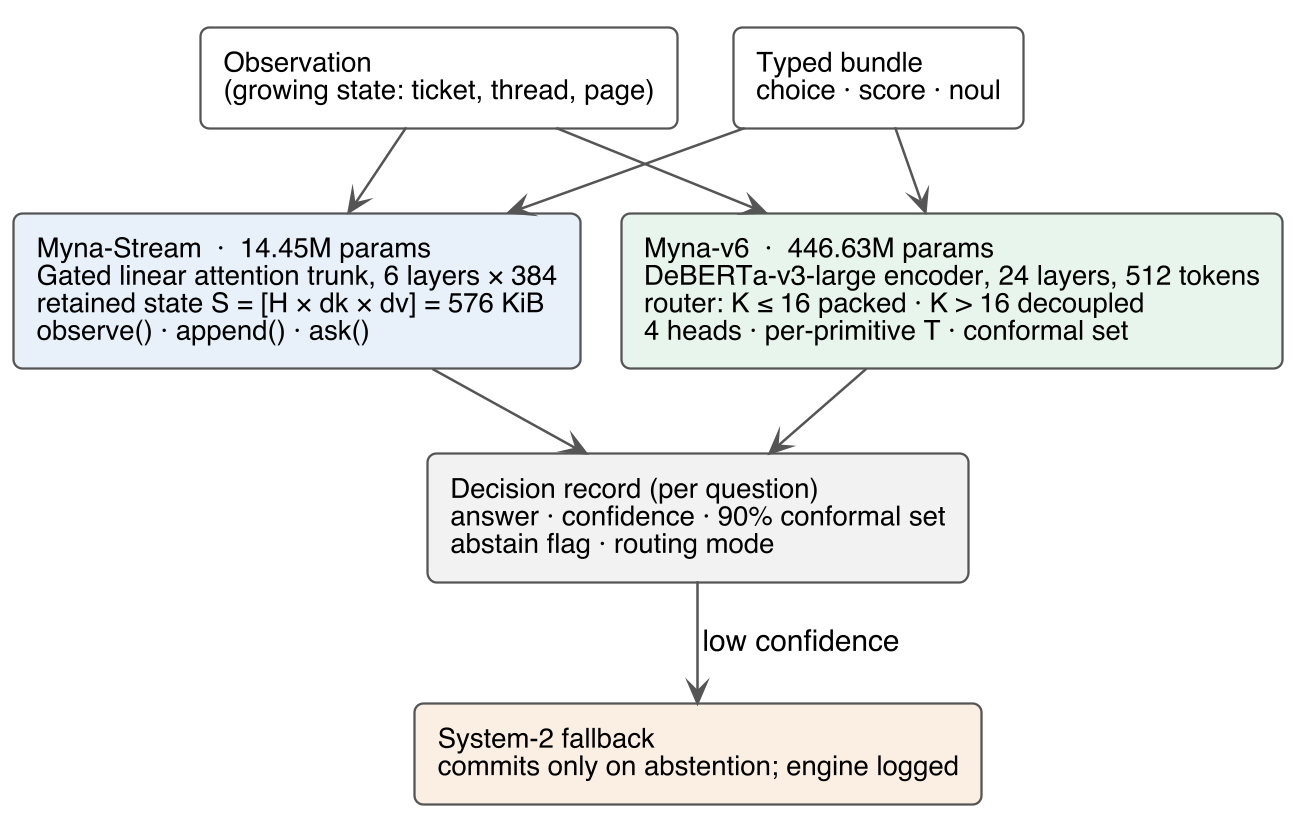
\includegraphics[width=0.82\linewidth]{fig1_architecture.png}
\caption{The two \myna{} engines behind one typed contract. \stream{} scans a growing observation
once into a 576 KiB state and answers from the cache; \vsix{} re-encodes the state on every
question and routes by option cardinality. Both write the same decision record, and a
low-confidence answer can be deferred to a second engine with the committing engine logged. The
figure is a schematic; the measurements are in Section~\ref{sec:systems}.}
\label{fig:arch}
\end{widefigure}

\begin{table}[t]
\centering
\footnotesize
\caption{The frozen \textsc{decision-v2-pilot} suite (11 public sources). Cells are the 16
$(\text{source},\text{question})$ pairs; $K$ is the number of options per question; the 78-option test questions carry the injected \textsc{none}-of-these option.}
\label{tab:dataset}
\begin{tabular}{lrrrr}
\toprule
Split & Rows & Questions & Cells & $K$ \\
\midrule
Train & 57{,}904 & 73{,}804 & 16 & 2--77 \\
Development & 1{,}176 & 1{,}440 & 16 & 2--78 \\
Calibration & 448 & 568 & 16 & 2--77 \\
\midrule
\multicolumn{5}{l}{\footnotesize The 448-row split is the suite's calibration partition; the 1{,}999-bundle}\\
\multicolumn{5}{l}{\footnotesize CAL draw used for temperatures is separate (Section~\ref{sec:calibration}).}\\
Test & 1{,}176 & 1{,}440 & 16 & 2--78 \\
\bottomrule
\end{tabular}
\end{table}

\section{Cardinality Is a Budget}
\label{sec:cardinality}

\subsection{The packed layout and its failure}
The packed scorer spends one sequence on the prefix, the state, and all option spans. Each span is
the option text, one \texttt{[MASK]}, and a separator. The state is truncated first, and if the
option spans still exceed the window, the fallback keeps a prefix of the options and collapses
the context to a single token. That fallback is not a graceful degradation: it deletes the state
and the tail options at the same time.

The budget was measured on every test cell with the suite's own renderer and tokenizer
(Figure~\ref{fig:cardinality}). The 15 non-banking77 cells have $K=2$--$15$; none overflows, and
every option receives a mask. The 77-way banking77 cell differs: mean option-span length is 490.3
tokens, or 6.36 tokens per option; with a median 25-token state, the total exceeds 512 on 50 of
116 rows. Across the cell the fallback keeps a mean of 75.9 options and drops up to 6, and on
overflow rows it also reduces the context to one token. The collapse is a budget failure, not a
tokenization artifact.

\subsection{An isolated routing ablation}
The router sends $K\le16$ to the packed scorer and $K>16$ to the set-aware head. The threshold is
a design cap, not a measured optimum: every cell at or below 15 options fits with zero drops, and
the only cell above the cap is the 77-way one. Sixteen leaves one option of headroom.

Because the router and the model changed between the two ablation arms, the routing
effect was re-measured on one checkpoint. The packed scorer was forced on every cell with
\texttt{-{}-max-packed 1000}, and the same weights were then scored with the router enabled.
Table~\ref{tab:routing} reports the result. Forcing the packed path scores 0.0345 on banking77
and 0.8222 macro; routing scores 0.6724 and 0.8620. The difference is $0.6379/16=0.0399$ macro,
and the other 15 cells are identical to the last digit, because the same weights take the same
path on them. This is a budget repair for exactly one cell.

\begin{widetable}
\centering
\footnotesize
\caption{The routing ablation on one checkpoint, same weights, same rows, same decoding. Only the
packed/decoupled switch changes. Every cell except banking77 is identical, so the macro difference
is one cell divided by sixteen.}
\label{tab:routing}
\begin{tabular}{lrrr}
\toprule
Arm & banking77 ($n=116$) & other 15 cells & 16-cell macro \\
\midrule
packed everywhere (\texttt{-{}-max-packed 1000}) & 0.0345 & 0.8747 & 0.8222 \\
routed ($K>16$ decoupled) & 0.6724 & 0.8747 & 0.8620 \\
\midrule
difference & $+0.6379$ & $0.0000$ & $+0.0399$ \\
\bottomrule
\end{tabular}
\end{widetable}

\subsection{The cost of routing}
Routing is not free. Under the packed path a question is one sequence; under the decoupled path it
is $K$ sequences, one per option. On the 77-way cell the decoupled path therefore runs 77 encoder
passes where the packed path runs one, and the measured cost follows: over six banking77
questions in one warm process, the median call is 4.90 s under the decoupled path and 0.43 s
under the packed path, a ratio of 11.4. The router buys accuracy on that cell at that price, and it is only
correct to pay it when the packed path has already failed. A deployment that routes on
cardinality alone pays it on every high-cardinality question, including ones the packed path
could have answered.

\subsection{What routing does not buy}
Routing is not a general accuracy method. The improvement is confined to the single cell whose
option spans do not fit, the other 15 cells are unchanged, and the representation is unchanged.
The result is a budget-allocation finding, not an architectural contribution, and it does not
support a broad accuracy claim.

\begin{widefigure}
\centering
\includegraphics[width=0.96\linewidth]{fig2_cardinality.pdf}
\caption{(a) The packed window is a budget: each point is a cell's median state plus option-span
tokens at its maximum $K$; the 77-way cell sits on the 512-token line. (b) The isolated routing
ablation: on one checkpoint, forcing the packed path scores 0.0345 on banking77 and enabling the
router scores 0.6724, with the other 15 cells identical.}
\label{fig:cardinality}
\end{widefigure}

\section{External Baselines and Comparison Footing}
\label{sec:baselines}

\subsection{The comparison set}
Table~\ref{tab:main} places the \myna{} arms beside five external references on the same 1{,}176
test bundles. Two are contemporary decision engines evaluated by their own released harnesses:
Laya 0.4.19, in three configurations, and VegaML 0.15.0. Both are third-party implementations
distributed with their own harnesses; we run each at its published default, record the version, and
report what the harness reports. Neither is a published method with a stated parameter count or
training corpus, so the paper treats them as engineering references rather than as literature
baselines, and Section~\ref{sec:related} positions the architectural comparison against published
readout families instead. Three further references are classical: a train-prior majority
classifier, a supervised TF-IDF unigram/bigram classifier with logistic regression, and a zero-shot
NLI scorer (\texttt{cross-encoder/nli-deberta-v3-small}).

The footing differs by arm, and the difference is large enough that it must travel with the
numbers. \vsix{} is fine-tuned on the suite's train split and is therefore in-domain on all 16
cells. The classical references are trained on the same split, so they are in-domain too. They predict
the cell's label directly from the state and the question, which is the standard formulation for a
text classifier; they do not score option strings, because a bag-of-words model has no
option-conditioned input. The comparison is therefore about the readout, not about access to
information: every arm sees the same state and the same question text.
Laya and VegaML are evaluated zero-shot: Laya's training mixture covers 6 of the 16 cells (the
five agnews cells and boolq), and VegaML is out-of-domain on all 16. The comparison is therefore
an in-domain fine-tuned encoder against two out-of-domain engines and three classical supervised
references, and no single column is a like-for-like statement about model quality.

\subsection{What the table shows}
\vsix{} reaches 0.8620 macro, 0.8632 overall, and 0.8393 joint bundle exact. The strongest
external reference is the supervised TF-IDF classifier at 0.7111 macro, 0.6840 overall, and
0.6293 bundle exact, followed by the best Laya configuration at 0.7050, 0.6792, and 0.6182.
VegaML 0.15.0 reaches 0.6160, the majority classifier 0.3726, and the zero-shot NLI scorer 0.3278.
The row-clustered 95\% interval on the \vsix{} macro is [0.8432, 0.8799]; the interval on joint
bundle exact is [0.8180, 0.8597]. The baselines' per-question records are not released in a form
that supports a paired interval, so their columns are point estimates.

The in-domain reference that matters is not TF-IDF but the same backbone. We fine-tuned
\texttt{microsoft/deberta-v3-large} on the same train split with a conventional readout: one linear
classifier per cell over the \texttt{[CLS]} of \texttt{state + question}. Trained for one epoch it
reaches 0.7126 macro over two seeds (0.7170 and 0.7082); trained for two epochs on seed 42 it
reaches 0.7746, and banking77 moves from 0.17 to 0.59. Most of the one-epoch result was therefore
underfitting, exactly as a training-schedule confound would predict.

\vsix{} leads the two-epoch control by 8.7 points, and the gap is now concentrated on multi-class
choice cells: dbpedia14 0.72 against 0.96, mnli 0.62 against 0.86, agnews/topic 0.69 against 0.91,
trec 0.73 against 0.95. On boolean cells and on yelp/recommend the two are within a few points.
Because the control improves monotonically with training, 8.7 points is an upper bound on what the
readout contributes, not a converged estimate; a longer schedule is the obvious next control and
the paper does not have it.

Pairing on the same rows makes the comparisons significant rather than descriptive. Resampling
bundles gives \vsix{} minus the per-cell classifier at $+0.0875$ macro (95\% CI $[0.0675,0.108]$;
McNemar on the 1{,}440 questions, $p=1.8\times10^{-22}$), minus Laya $+0.196$ $[0.169,0.222]$ and
minus VegaML $+0.246$ $[0.218,0.275]$. The TF-IDF arm has no per-question record in the release, so
its interval is not computed; that is a gap in the artifact, not in the test. The paired effect
sizes are moderate rather than marginal: Cohen's $d$ is 0.27 against the per-cell classifier, 0.44
against Laya and 0.51 against VegaML on 1{,}440 paired questions.

\vsix{} also leads the supervised TF-IDF classifier on 15 of the 16 cells and loses
\texttt{banking77/intent}, 0.6724 against 0.8190: a bag-of-words classifier that sees the whole
option list beats the routed set-aware head on the 77-way question.

\begin{widetable}
\centering
\footnotesize
\caption{All arms on the same 1{,}176 bundles and 1{,}440 questions. Macro is the unweighted mean
over the 16 cells; bundle exact is the fraction of bundles in which every question is correct.
Laya is in-domain on 6 of 16 cells and zero-shot on 10; VegaML is zero-shot on all 16; \vsix{} is
in-domain on all 16. The two \myna{} rows differ only in the routing switch.}
\label{tab:main}
\begin{tabular}{lrrrr}
\toprule
Arm & macro & overall & bundle & footing \\
\midrule
Myna v6, routed & \textbf{0.8620} & 0.8632 & 0.8393 & in-domain \\
Myna v6, packed everywhere & 0.8222 & 0.8118 & 0.7764 & in-domain \\
TF-IDF + logistic regression & 0.7111 & 0.6840 & 0.6293 & in-domain, text only \\
DeBERTa-v3-large, per-cell classifier & 0.7746 & 0.7514 & 0.7049 & in-domain, same backbone (2 epochs) \\
Laya 0.4.19 (typed-decisions best) & 0.7050 & 0.6792 & 0.6182 & 6/16 in-domain \\
Laya 0.4.19 (raised + tournament) & 0.6829 & 0.6597 & 0.5918 & 6/16 in-domain \\
Laya 0.4.19 (English default) & 0.6624 & 0.6333 & 0.5595 & 6/16 in-domain \\
VegaML 0.15.0 & 0.6160 & 0.5833 & 0.5119 & zero-shot \\
Train-prior majority & 0.3726 & 0.2965 & 0.2041 & in-domain \\
Zero-shot NLI & 0.3278 & 0.3465 & 0.3027 & zero-shot \\
\bottomrule
\end{tabular}
\end{widetable}

\begin{widefigure}
\centering
\includegraphics[width=0.90\linewidth]{fig3_external.pdf}
\caption{All ten arms on the same 1{,}176 test bundles. Bars are 16-cell macro; diamonds are
joint bundle exact. The ordering is stable under both aggregates. The Myna row is in-domain and
the two decision engines are out-of-domain or zero-shot on most cells, so the figure ranks
performance on this suite, not model quality in general.}
\label{fig:external}
\end{widefigure}

\section{Bundle Consistency: An Observed Property}
\label{sec:consistency}

A bundle can contradict itself: an article can be labelled ``sports'' while the answer to ``is
this article about sports?'' is ``no''. The suite contains 172 bundles that ask both questions:
92 agnews bundles with a topic question and two of the four class booleans, and 80 yelp bundles
with a star rating and a recommendation question.

The checkpoint's summary records 0/172 contradictions. That record is reproducible: the rule that
produced it is in the released notebook's graph-ablation cell, and
re-implemented as code it gives 0/172 for \vsix{}, 1/172 for Laya, and 2/172 for VegaML. The rule
is narrow. It counts a bundle only when the bundle carries both a \texttt{choice} and a
\texttt{noul} question, the predicted option text appears inside the boolean question, and the
boolean is answered ``no''. It cannot see a yelp rating/recommendation contradiction, because the
rating is a \texttt{score} question, and it misses any pair whose option text is not a substring
of the question.

This paper therefore reports two numbers: the notebook rule, and a broader predicate that covers
both sources. A bundle is a contradiction under the broader predicate iff
the predicted topic is class $c$, the bundle asks \texttt{is}$\_c$, and the answer is ``no''; or
the predicted rating is 4--5 while \texttt{recommend} is ``no'', or 1--2 while \texttt{recommend}
is ``yes''. Under it, \vsix{} has 3 contradictions in 172 bundles, Laya has 10, and VegaML has 29
(Table~\ref{tab:consistency}). The \vsix{} rate is 1.7\%, and the three errors are two agnews
bundles and one yelp bundle. The yelp half of the rule is strict --- a 4-star review that advises
against the venue is counted as a contradiction --- so we report the halves separately: agnews
2/92 for \vsix{} against 5/92 (Laya) and 26/92 (VegaML), yelp 1/80 against 5/80 and 3/80. The
ranking is the same in both halves, and the yelp counts are small enough that the strict rule does
not drive the result.

This is a property of the fine-tuned encoder, not of the architecture. The checkpoint stores a
cross-question graph head, but it changes nothing: the released notebook's five-arm ablation
(scorer-only, graph-full, gate-zero, shuffled, and exact factor-graph decoding) returns the same
accuracy, 0.8899, and the same 1/172 contradictions for every arm on its 172 multi-question
development bundles, and the test arms differ by one question in 436. The inference path never calls the module, and no consistency term
was trained: the training config defines a consistency weight that no cell reads, and the training
loop minimizes per-question cross-entropy. The paper therefore makes
no claim that the architecture enforces consistency, and it does not present the measurement as a
methodological contribution. It is a descriptive statistic
that a deployment can monitor, and it is the statistic on which \vsix{} has its largest margin
over the two external engines.

\begin{table}[t]
\centering
\footnotesize
\caption{Bundle consistency, same 172 bundles, under the notebook's recovered rule and under the
broader released predicate. The notebook column re-implements that rule and reproduces the
published 0/172 for Myna; the released column also counts the yelp rating/recommendation pair that
the notebook rule cannot see.}
\label{tab:consistency}
\begin{tabular}{lrrrr}
\toprule
Engine & notebook rule & released predicate & agnews & yelp \\
\midrule
Myna v6 & 0/172 & 3/172 & 2 & 1 \\
Laya 0.4.19 & 1/172 & 10/172 & 5 & 5 \\
VegaML 0.15.0 & 2/172 & 29/172 & 26 & 3 \\
\bottomrule
\end{tabular}
\end{table}

\section{Calibration, Selective Prediction, and Conformal Sets}
\label{sec:calibration}

\subsection{Temperature scaling and calibration error}
The checkpoint stores three temperatures, 0.9 for \texttt{choice}, 0.9 for \texttt{score}, and
0.85 for \texttt{noul}, fitted per primitive by minimizing negative log-likelihood on the CAL split
that the released notebook draws from the training pool. The rebuilt split is committed
with the paper (\texttt{runs/cal\_split.jsonl}; 1{,}999 bundles, 2{,}548 questions,
SHA-256 \texttt{918ddbf2\ldots0202a}); the original file is not recoverable, so
this is a definition-level reproduction, not a byte match of the lost file. They produce zero argmax flips between
development and test, so the calibration step changes probabilities but not decisions. On the
1{,}440 test questions the 10-bin expected calibration error is 0.0190 and the multiclass Brier
score is 0.0449. The ECE is stable in the bin count --- 0.0184 at 5 bins, 0.0190 at 10, 0.0213 at
15, 0.0223 at 20, 0.0276 at 30 --- and equal-frequency (adaptive) bins give 0.0162 at 10 bins, so
the headline value is not an artefact of one binning; the original run recorded 0.0189 and 0.0434, and the small gap is the rendering
difference between its pipeline and the released engine. Figure~\ref{fig:calibration}a is the
reliability diagram. The largest bin holds 847 questions at mean confidence 0.980 and accuracy
0.983; the mid-confidence bins track the diagonal closely, with the 0.6--0.7 bin at mean
confidence 0.647 and accuracy 0.681.

\subsection{Selective prediction}
Selective prediction is a curve, not a point. Ranking the 1{,}440 test questions by top probability
gives accuracies of 0.9889 at 50\% coverage, 0.9815 at 60\%, 0.9633 at 70\%, 0.9358 at 80\%, and
0.9035 at 90\%. The curve is monotone in the required direction: abstaining on the least confident
questions buys accuracy at every operating point measured. The original run reported 0.9873 at 60\%
coverage; our top-probability re-ranking of the same released outcomes gives 0.9815, and the
0.58-point difference is not resolved, because the original selective routine is not released.
The v0 streaming arm, on the same calibration split, reaches a maximum of 0.596 at 10.0\% coverage
and fails the same target; the confidence mechanism is a property of the \vsix{} arm, not of the
architecture family.

\subsection{Conformal prediction: what fails, and why}
\label{sec:conformal}

We report three calibrations of the same nonconformity score, Eq.~\eqref{eq:conformal}, on the same
test questions. \emph{Released}: the per-primitive quantiles stored in the checkpoint, fitted on the
the 568-question calibration split. \emph{Refit}: one pooled quantile fitted on the rebuilt
2{,}548-question CAL split. \emph{Mondrian}: one quantile per
cell on the same rebuilt split, the cell-conditional calibration of Vovk \cite{vovk2012conditional}, which is the standard answer when
exchangeability across heterogeneous questions is in doubt.

\begin{center}
\footnotesize
\begin{tabular}{lrrl}
\toprule
 & 90\% & 95\% & calibration \\
\midrule
released (per primitive, 568 questions) & 0.8368 & 0.9333 & 568 \\
refit per primitive (2{,}548) & 0.8694 & 0.9396 & shared \\
refit, disjoint halves (2{,}548) & 0.8729 & 0.9354 & half/half \\
refit pooled (2{,}548) & 0.8917 & 0.9437 & shared \\
Mondrian per cell (2{,}548) & 0.8396 & 0.9215 & shared \\
\midrule
nominal & 0.90 & 0.95 & \\
\bottomrule
\end{tabular}
\end{center}

Fitting the temperature on one half of the CAL bundles and the quantile on the other, so that the
scoring function is fixed independently of the calibration examples, moves coverage by 0.35 points
at the 90\% target (86.94\% to 87.29\%) and 0.42 at 95\% (93.96\% to 93.54\%): the shared-split
design is not what drives the shortfall.

Two things follow, and neither is the story the earlier draft told. First, most of the 90\% shortfall
is calibration-sample size, not a violated guarantee: refitting the same score on 2{,}548 questions
moves coverage from 83.68\% to 89.17\%, within a point of nominal. Second, cell-conditional
calibration does not help — it is worse than pooled refitting at both levels (83.96\% and 92.15\%),
because the per-cell calibration sets are ten times smaller and the residual violation is
\emph{within} a cell, not between cells: dbpedia14 covers 68.97\% at the 90\% target while
agnews/is\_business covers 90.70\%, and both are conditioned on their own cell. Stratifying by the
cell therefore does not restore exchangeability; it only shrinks the sample each quantile is fitted
on.

The honest conclusion is narrower than ``conformal fails'' and more useful. A marginal guarantee is
not available on this suite for two independent reasons — calibration and test differ in source mix,
and questions within a bundle share a state and are dependent — and a cell-conditional fit does not
repair either, because the dependence is inside the cell's own distribution. The paper therefore
does not use conformal sets as a coverage guarantee or as the abstention method; the selective
results above use temperature-scaled confidence and the risk--coverage curve. The engine still
exposes a 90\% set as a ranking signal, with no coverage claim attached; a deployment that needs a
calibrated threshold should fit it on its own traffic.

\begin{widetable}
\centering
\footnotesize
\caption{Calibration and selective prediction on the 1{,}440 test questions, recomputed from the
released per-question records. The released conformal quantiles under-cover; refitting on the
larger calibration split closes most of the gap, and cell-conditional calibration does not.}
\label{tab:calibration}
\begin{tabular}{lr}
\toprule
Metric & Value \\
\midrule
ECE (10 bins) & 0.0190 \\
Brier (multiclass) & 0.0449 \\
selective accuracy @ 50\% coverage & 0.9889 \\
selective accuracy @ 60\% coverage & 0.9815 \\
selective accuracy @ 70\% coverage & 0.9633 \\
selective accuracy @ 80\% coverage & 0.9358 \\
selective accuracy @ 90\% coverage & 0.9035 \\
conformal 90\%, released quantiles & 0.8368 \\
conformal 95\%, released quantiles & 0.9333 \\
conformal 90\%, refit on 2{,}548 & 0.8917 \\
conformal 95\%, refit on 2{,}548 & 0.9437 \\
conformal 90\%, Mondrian per cell & 0.8396 \\
conformal 95\%, Mondrian per cell & 0.9215 \\
\bottomrule
\end{tabular}
\end{widetable}

\begin{widefigure}
\centering
\includegraphics[width=0.94\linewidth]{fig4_calibration.pdf}
\caption{(a) Reliability on the 1{,}440 test questions, 10 bins; marker area is bin count. (b)
Risk--coverage on the same ranking. (c) Nominal versus empirical conformal coverage: 83.68\% at
90\% and 93.33\% at 95\%.}
\label{fig:calibration}
\end{widefigure}

\section{Systems: Constant State and Deployment}
\label{sec:systems}

\subsection{Latency with a constant state}
On one Apple M5, in one process, with the same state and question dictionary, \stream{} answers
33.08 ms at one question, 74.87 ms at five, 120.75 ms at ten, and 869.95 ms at fifty end-to-end.
With the state already cached, the ask-only path is 14.86 ms at one question, 55.45 ms at five,
98.22 ms at ten, and 787.12 ms at fifty. Ask is 10.1 ms fixed plus 9.6 ms per question with a
state slope of $-10.3$ $\mu$s/token, the fixed-size state measured; observe is 360 $\mu$s/token.
The ask-only path is the same engine with the scan removed, not a second model.

\subsection{MLX and the browser}
The same 14.45M checkpoint ports to MLX over identical weights, with no conversion step. MLX fp32
is 1.76--2.40$\times$ faster than PyTorch MPS from 128 to 16{,}384 state tokens; MLX int8 is
1.79--2.75$\times$ and 17.40 MiB on disk against 55.13 MiB. The ONNX export runs in Chrome 153
under WebAssembly at 59.32 MiB artifact, 73.09 MiB on the wire, a 394.4 ms cold load, and a 435.8
ms p50 for a three-decision session; all six parity checks pass, and the maximum probability drift
against the torch engine is $1.03\times10^{-6}$. The export's own parity check is
$8.94\times10^{-8}$ on the decision output.

\subsection{Why int8 is not deployed}
int8 is 3.17$\times$ smaller and not faster. Five of the six linear shapes this model uses are
slower quantized (0.43--1.06$\times$ fp32/int8) even though int8 reads 3.6$\times$ fewer weight
bytes, because the quantized pass gets 10--37 GB/s of weight read against fp32's 55--257 GB/s on
the same box. It is also not faithful: on 20 real questions the MLX int8 port moves option
probabilities by 9.24e-3 and flips one argmax on a question whose top two options were 0.0008
apart; the ONNX int8 artifact drifts 6.48e-2 and fails five browser checks. The fp32 path is deployed on
both routes, and the int8 artifacts remain in the tree for byte-constrained uses rather than for
speed.

\subsection{Two engines, one API}
The systems numbers are \stream{}'s, not \vsix{}'s. \vsix{} has no ONNX export and no browser
build, and it re-encodes the state, so a latency number for it would be a different experiment.
The shared API is what makes the split usable: an application can run \stream{} for high-frequency
decisions and defer to \vsix{} or another second-tier model on abstention, with the committing
engine logged. No end-to-end cascade accuracy is claimed, because no joint deferral policy was
trained.

\begin{widetable}
\centering
\footnotesize
\caption{Systems measurements on one Apple M5. Latency is p50, 10 repetitions, 3 warm-ups, same
process, same inputs. The MLX and browser rows are the 14.45M streaming arm, not \vsix{}.
``Cached'' is the ask-only path of the same engine.}
\label{tab:systems}
\begin{tabular}{ll}
\toprule
Metric & Value \\
\midrule
parameters & 14{,}449{,}280 \\
retained state & 576 KiB (589{,}824 B) at every length \\
end-to-end latency & 33.08 / 74.87 / 120.75 / 869.95 ms at 1 / 5 / 10 / 50 questions \\
ask-only latency & 14.86 / 55.45 / 98.22 / 787.12 ms at 1 / 5 / 10 / 50 questions \\
MLX fp32 vs MPS & 1.76--2.40$\times$; artifact 55.13 MiB \\
MLX int8 vs MPS & 1.79--2.75$\times$; artifact 17.40 MiB; 9.24e-3 drift, 1 argmax flip \\
ONNX browser & 59.32 MiB artifact, 394.4 ms cold, 435.8 ms p50, 1.03e-6 drift \\
ONNX int8 & 18.56 MiB; 6.48e-2 drift; 5 browser checks fail \\
\bottomrule
\end{tabular}
\end{widetable}

\begin{widefigure}
\centering
\includegraphics[width=0.94\linewidth]{fig5_systems_ours.pdf}
\caption{(a) p50 latency against the number of questions per request, same box and inputs; the
cached curve is the ask-only path of the same engine. (b) MLX fp32 and int8 against PyTorch MPS
over state lengths. (c) Artifact size; int8 is smaller but not faster and not faithful.}
\label{fig:systems}
\end{widefigure}

\section{The Streaming Arm: Compute, Not Accuracy}
\label{sec:diagnostics}

The streaming arm is a deployment result. This section states its accuracy limits once, so that no
reader mistakes the systems numbers of Section~\ref{sec:systems} for a benchmark claim.

\textbf{It does not learn the 16-cell suite.}
The v1b checkpoint scores 0.4893 macro on the real suite against a 0.4331 majority floor, and its
data-path variant 0.5339. A checkpoint trained on the synthetic typed-decision task scores 0.9525
there and 0.3423 on the synthetic rows of the real suite, below that suite's 0.3546 floor: success
on the synthetic task does not transfer.

\textbf{Long context is flat at chance.}
The 4k truncated-backprop arm scores 0.1833 at 4{,}096 state tokens and 0.1500 at 16{,}384; the
128-token rung is also 0.1500 against a 0.167 uniform floor. Steps 799 and 1199 agree exactly on all
three shared rungs, so the limiter is the mechanism rather than the training dose. This is not a
decay curve: the model never learned the task at any length.

\textbf{Why the systems numbers still mean something.}
Latency, memory and numerical drift are properties of the scan and the state size, not of the
weights' quality: a constant-state layer costs what Eq.~\eqref{eq:state} costs, whatever the
checkpoint has learned. The measurements in Section~\ref{sec:systems} are reported for that reason
and are not offered as evidence that the architecture is competitive. Closing the accuracy gap is
future work, and the paper makes no cascade claim: no deferral policy between the engines was
trained or evaluated.

\begin{widetable}
\centering
\footnotesize
\caption{The small-engine accuracy diagnostics. Synthetic and real columns are different suites.
These rows bound the streaming prototype; they are not comparison arms.}
\label{tab:diagnostics}
\begin{tabular}{llrr}
\toprule
Arm & Data & macro & note \\
\midrule
v0 & synthetic & 0.9525 & gate 0.94 \\
v1b & synthetic & 0.3423 & below floor \\
v1b & real suite & 0.4893 & floor 0.4331 \\
data-path v1b & real suite & 0.5339 & \\
v6 (reference) & real suite & 0.8620 & in-domain \\
lc1-4k, 4k state & needle & 0.1833 & floor 0.167 \\
lc1-4k, 16k state & needle & 0.1500 & floor 0.167 \\
\bottomrule
\end{tabular}
\end{widetable}

\section{Discussion and Limitations}
\label{sec:limitations}

\textbf{Pre-training exposure.}
\texttt{deberta-v3-large} was pre-trained on a web corpus that overlaps several sources used here
(agnews, imdb, sst, yelp among them), so the in-domain numbers may benefit from exposure during
pre-training. The suite is not a contamination-free evaluation, and the external engines are not on
an equal exposure footing either. A clean measurement would use sources that post-date the backbone;
this one does not, and the paper flags it rather than correcting for it.

\textbf{Scope and footing.}
This is a controlled study on one frozen suite. The reported intervals are sampling error over the
1{,}176 rows of the split, not a population over checkpoints or datasets. The accuracy arm is
fine-tuned on the suite's train split, so all 16 cells are in-domain, while the two external
engines are out-of-domain on at least 10 cells and the NLI scorer is zero-shot. The paper
therefore does not claim out-of-domain generalization or state-of-the-art superiority. A second
training seed, an out-of-domain cell set, and a paired harness for the external engines are the
three measurements that would most strengthen the claims, and none is in this draft.

\textbf{The ordinal primitive.}
The \texttt{score} cells are the engine's weakest group and its most ordinary: 0.6375 on
amazon/stars, 0.6125 on sst5/sentiment, and 0.6250 on yelp/rating, against a 0.20 uniform floor and
a 0.525 TF-IDF baseline on the first. The checkpoint also stores a CORAL \cite{cao2020coral} ordinal head that the
released configuration disables; it was trained with cross-entropy plus a cumulative-link term and
an earth-mover term, and gated on development accuracy against the packed head's 0.6542. We decoded
the stored head with the notebook's own forward pass and scored it on the same 240 questions
(released with the paper): it reaches 0.6333 on the three cells against 0.6292 for the packed
head, with 7 questions won and 6 lost on a paired comparison. The head is a wash, which is
consistent with the decision to leave it off, and the ordinal cells are simply harder
than the boolean cells rather than broken.

\textbf{What could not be verified.}
The training notebooks are released (\texttt{release/notebooks/}): the v5 loop, the
development-split temperature fit, the per-option banking77 head, and the v6 run with its CAL
split, its CAL temperature and conformal fit, the CORAL gate, and the cell that writes
\texttt{myna-v6-unified.pt}. The CAL file itself was not committed. It is redrawn by
\texttt{release/build\_cal\_split.py} (seed 42, proportional per source), which yields 1{,}999
bundles and 2{,}548 questions; the model card's 2{,}000 is the rounding target, and the rebuild is
a definition-level reproduction rather than a hash of the lost file. The suite's committed
calibration split has 448 rows and 568 questions and is a different, earlier split. The banking77 \texttt{none\_absent} decomposition is 0/12 here against 7/12 in the
training record, while the cell aggregate matches at 78/116 against the recorded 77/116.
\vsix{}'s 512-token maximum also puts the long-context question out of its reach. These gaps are
reported rather than reconstructed.

\textbf{Data and code availability.}
The frozen suite, the checkpoint, the per-question records for every \myna{} arm, both consistency
predicates, the four training notebooks, the CAL-split builder, the reference training
implementation, and every table and figure generator are released with the paper. The four
training notebooks are in \texttt{release/notebooks/} with digests; the reference trainer
reproduces the architecture and objective, loads into the engine, and matches it token-for-token.
Bit-exact reproduction of the original optimisation trajectory is not claimed, because the run
depends on hardware and library versions that the notebooks record but do not pin.

\textbf{Reproducibility statement.}
Every number in this paper is recomputed from committed per-question records by one aggregation
script, and the repository's registry re-derives each quoted figure from its witness
($49$ rows, $205$ figures, one gated for lack of a witness). The frozen suite, the rebuilt
calibration split with its SHA-256, the four training notebooks with digests, the consistency
predicates, the reference trainer, the routing-cost and conformal harnesses, and the figure
generators are all released. A container recipe builds the environment and runs the aggregation
with no GPU. What is not claimed is bit-exact reproduction of the original training trajectory,
because the run depends on hardware and library versions that the notebooks record but do not pin;
and one artifact the reviewers asked for, per-question TF-IDF outcomes, is not in the release.

\textbf{Ethics.}
Typed decisions are used in routing, moderation, and triage. An abstention flag is not a safety
guarantee: the confidence scores are not certified, the suite is English and public, and the labels
carry their sources' biases. A deployment should log the committing engine and keep a human in the
loop for high-stakes cells. Two failure modes deserve naming: misrouting a moderation or triage
item at 33--870\,ms is fast enough to remove human review from the loop by default, and the suite is
English-only, drawn from public corpora whose demographic coverage is uneven, so error rates across
groups are unmeasured here. No fairness audit was run; a deployment should not infer one from the
aggregate numbers. This study measured latency and bytes, not energy.

\textbf{Funding.} This research received no external funding.

\textbf{Competing interests.} The authors declare no competing interests.

\textbf{Author contributions.} Aashish Kumar Mahato (first and corresponding author):
conceptualization, methodology, software,
validation, formal analysis, investigation, data curation, writing---original draft, and
visualization. Prakrist Dhakal: software (the paired-bootstrap harness and the VegaML control
run), validation, and writing---review and editing.

\section{Conclusion}
\label{sec:conclusion}

This paper reported a measurement study of a typed decision engine on a frozen 16-cell suite,
against two contemporary decision engines and three classical baselines. The accuracy arm reaches
0.8620 macro, 0.8632 overall, and 0.8393 joint bundle exact; the strongest external reference, a
supervised TF-IDF classifier, reaches 0.7111 macro, and the best external decision engine reaches
0.7050. The lead is carried by the choice and boolean cells; the ordinal cells sit near 0.63, and a
disabled ordinal head does not improve them.

Three further results are bounded. Cardinality routing is a budget repair worth 0.0399 macro on
exactly one cell, and it multiplies the encoder passes on that cell by the option count.
Cross-question consistency is an observed property of the encoder (3/172 against 10/172 and 29/172
for the external engines), not an enforced constraint; the graph head that would enforce it does not
change any answer. Split-conformal sets cover 83.68\% at a 90\% target, so the paper reports
calibration error and risk--coverage instead of a coverage guarantee.

What remains is scope. The suite is one frozen split, the accuracy arm is in-domain, and the
external engines are not. The in-domain baseline is one epoch and visibly underfits the 77-way
cell, so its 8.7-point gap is an upper bound on the readout's advantage. An out-of-domain cell set
and a longer baseline schedule are the measurements that would extend these claims, and the paper
says so rather than implying otherwise.

\bibliographystyle{elsarticle-num}
\bibliography{refs}
\clearpage
\appendix

\section{Reproduction and Artifact Map}
\label{app:extra}

Every number in this paper is read from a committed JSON artifact or recomputed by a script in the
repository. The main commands are:

{\scriptsize
\begin{verbatim}
python -m bench.v6_audit --ckpt "myna-v5-prototype 2" \
  --split test --every 1 \
  --out runs/paper_v6_audit.json --md runs/paper_v6_audit.md \
  --metrics runs/paper_v6_test.metrics.json \
  --rowout runs/paper_myna_v6_test.rowoutcomes.json
python -m bench.v6_audit --ckpt "myna-v5-prototype 2" \
  --split test --every 1 \
  --max-packed 1000 --out runs/v6_packed_forced.json \
  --rowout runs/v6_packed_forced.rowoutcomes.json
python -m bench.paper_numbers --out runs/paper_numbers.json
python -m bench.consistency_audit \
  --out runs/consistency_audit.json
python -m bench.paper_bootstrap --out runs/paper_bootstrap.json
python -m bench.routing_cost --out runs/routing_cost.json
python -m bench.prob_dump --split test \
  --out runs/v6_prob_test.jsonl
python paper/make_figures_v2.py
\end{verbatim}
}

The routed re-score takes 953 s on CPU for all 1{,}176 bundles and writes all 1{,}440 question
outcomes; the packed-forced arm takes 540 s. \texttt{bench/paper\_numbers.py} recomputes macro,
overall accuracy, joint bundle exact, the per-cell table, per-primitive accuracy, ECE, Brier, and
the risk--coverage curve from those records, and refuses a record whose correctness flag disagrees
with its own prediction and gold. The row-clustered intervals use 20{,}000 bootstrap replicates with
seed 20261104 and resample rows, not questions, because the questions of a bundle share a state.

The witnesses are, one per line:
{\footnotesize\ttfamily\raggedright
runs/paper\_v6\_audit.json \\
runs/paper\_v6\_test.metrics.json \\
runs/paper\_myna\_v6\_test.rowoutcomes.json \\
runs/v6\_packed\_forced.* \\
runs/paper\_numbers.json \\
runs/paper\_bootstrap.json \\
runs/routing\_cost.json \\
runs/consistency\_audit.json \\
runs/paper\_cell\_intervals.json \\
runs/external\_\{majority,tfidf,nli\}.json \\
runs/laya\_0419\_test.rowoutcomes.json \\
runs/vegaml\_0150\_test.rowoutcomes.json \\
runs/latency\_matched.json \\
runs/bench\_mlx\_int8.json \\
runs/browser\_g3.json \\
runs/g6\_* and runs/needle\_* \\
\par}

\paragraph{Known gaps.}
Four training notebooks are in \texttt{release/notebooks/} with their digests: three copies of the
v5 run (training loop, development-split temperature fit, per-option banking77 head, checkpoint
merge) and the v6 run (CAL split, CAL temperature and conformal fit, CORAL gate, checkpoint
assembly). The original CAL file was not committed; the deterministic redraw (1{,}999 bundles,
2{,}548 questions) is now a committed artifact with its SHA-256, and
\texttt{release/build\_cal\_split.py} regenerates it. The suite's committed calibration
split has 448 rows and 568 questions and is a different, earlier split; no number in this paper is
computed from it. The banking77 \texttt{none\_absent}
decomposition is 0/12 here against 7/12 in the training record while the cell aggregate matches at
78/116. These gaps are reported rather than reconstructed.

\section{Per-Cell Results}
\label{app:cells}

Table~\ref{tab:cells} reports the corrected per-cell re-score with row-clustered intervals.

\begin{widetable}
\centering
\footnotesize
\caption{Per-cell corrected re-score with row-clustered 95\% intervals (5{,}000 replicates for the per-cell intervals; 20{,}000 for the macro intervals, seed
20261104). The interval is on the cell accuracy; the unit resampled is the row, not the question.}
\label{tab:cells}
\begin{tabular}{lrrr}
\toprule
Cell & $n$ & Myna & 95\% CI \\
\midrule
agnews/is\_business & 43 & 0.9535 & [0.8837, 1.0000] \\
agnews/is\_scitech & 49 & 0.9184 & [0.8367, 0.9796] \\
agnews/is\_sports & 47 & 0.9787 & [0.9362, 1.0000] \\
agnews/is\_world & 45 & 1.0000 & [1.0000, 1.0000] \\
agnews/topic & 116 & 0.9052 & [0.8448, 0.9569] \\
amazon/stars & 80 & 0.6375 & [0.5250, 0.7375] \\
banking77/intent & 116 & 0.6724 & [0.5862, 0.7500] \\
boolq/answer & 80 & 0.8500 & [0.7750, 0.9250] \\
contrastive/decision & 196 & 0.9847 & [0.9643, 1.0000] \\
dbpedia14/category & 116 & 0.9569 & [0.9138, 0.9914] \\
imdb/positive & 80 & 0.9625 & [0.9125, 1.0000] \\
mnli/relation & 116 & 0.8621 & [0.8017, 0.9224] \\
sst5/sentiment & 80 & 0.6125 & [0.5125, 0.7250] \\
trec/answer\_type & 116 & 0.9483 & [0.9052, 0.9828] \\
yelp/rating & 80 & 0.6250 & [0.5125, 0.7375] \\
yelp/recommend & 80 & 0.9250 & [0.8625, 0.9750] \\
\bottomrule
\end{tabular}
\end{widetable}

The three ordinal cells are the only cells below 0.6, and they are the cells on which the corrected
harness changes the answer. The five agnews boolean cells and the contrastive cell are above 0.95.

\section{Decision Sequence and Diagnostics}
\label{app:sequence}

Figure~\ref{fig:sequence} gives the call sequence for one bundle. The readout is per question; no
cross-question constraint is applied. Figure~\ref{fig:diagnostics} plots the small-engine
diagnostics of Section~\ref{sec:diagnostics}.

\begin{widefigure}
\centering
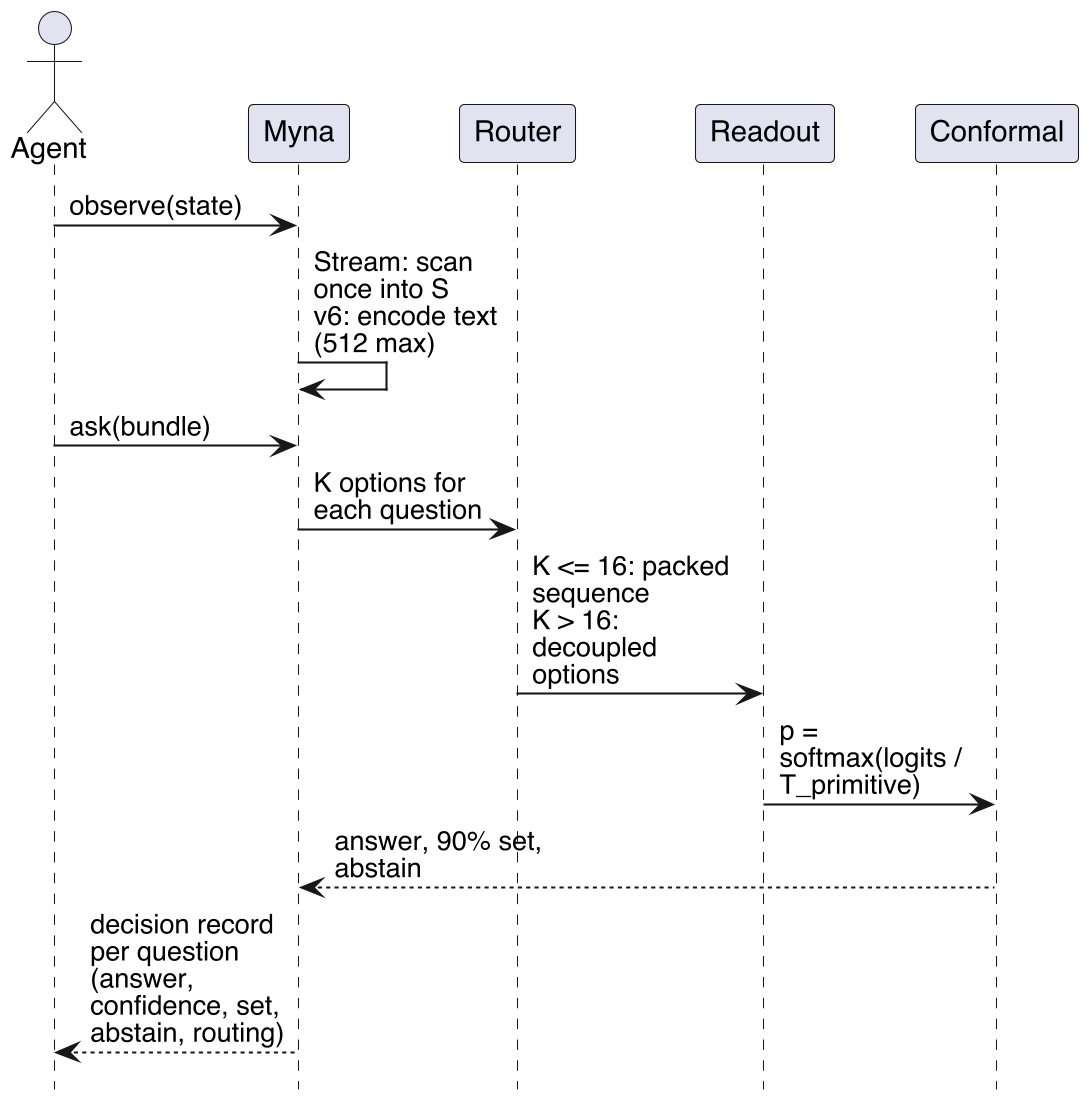
\includegraphics[width=0.72\linewidth]{fig7_sequence.png}
\caption{The \myna{} decision sequence for one bundle. The router chooses packed scoring for
$K\le16$ and decoupled scoring for $K>16$. The conformal gate can attach a 90\% set; this paper
does not use it as a coverage guarantee.}
\label{fig:sequence}
\end{widefigure}

\begin{widefigure}
\centering
\includegraphics[width=0.94\linewidth]{fig6_diagnostics_journal.pdf}
\caption{(a) Synthetic versus real-suite macro for the streaming arms. The dashed line is the 0.94
synthetic gate; the dotted line is the 0.433 majority floor. (b) Needle accuracy against state
length for the 4k-trained arm: flat at the 0.167 uniform floor.}
\label{fig:diagnostics}
\end{widefigure}

\begin{widetable}
\centering
\footnotesize
\caption{Per-cell accuracy on the 1{,}176 test bundles: \vsix{}, the same-backbone per-cell
classifier (seed 21, six epochs, the converged control) and the supervised TF-IDF reference. The
last column is the classifier minus \vsix{}.}
\label{tab:percell_baselines}
\begin{tabular}{lrrrr}
\toprule
Cell & \vsix{} & DeBERTa per-cell & TF-IDF & $\Delta$ (DeBERTa $-$ \vsix{}) \\
\midrule
agnews/is\_business & 0.9535 & 0.9302 & 0.8372 & -0.0233 \\
agnews/is\_scitech & 0.9184 & 0.9796 & 0.8571 & +0.0612 \\
agnews/is\_sports & 0.9787 & 1.0000 & 0.9362 & +0.0213 \\
agnews/is\_world & 1.0000 & 0.9778 & 0.9556 & -0.0222 \\
agnews/topic & 0.9052 & 0.6897 & 0.7931 & -0.2155 \\
amazon/stars & 0.6375 & 0.5625 & 0.5250 & -0.0750 \\
banking77/intent & 0.6724 & 0.6293 & 0.8190 & -0.0431 \\
boolq/answer & 0.8500 & 0.7875 & 0.6125 & -0.0625 \\
contrastive/decision & 0.9847 & 0.8724 & 0.5663 & -0.1122 \\
dbpedia14/category & 0.9569 & 0.7155 & 0.8448 & -0.2414 \\
imdb/positive & 0.9625 & 0.9625 & 0.8500 & +0.0000 \\
mnli/relation & 0.8621 & 0.7155 & 0.4052 & -0.1466 \\
sst5/sentiment & 0.6125 & 0.6250 & 0.3750 & +0.0125 \\
trec/answer\_type & 0.9483 & 0.7414 & 0.7759 & -0.2069 \\
yelp/rating & 0.6250 & 0.5750 & 0.4375 & -0.0500 \\
yelp/recommend & 0.9250 & 0.9250 & 0.7875 & +0.0000 \\
\bottomrule
\end{tabular}
\end{widetable}


\end{document}